
\section{Background}\label{sec:background}
\iffalse
\begin{table*}[tb]\centering
    \caption{Sample Caption}
    %\scriptsize
    \begin{tabular}{l r r r r r r r}%
        \toprule
        \textbf{App} & \textbf{NSGA-II} & \textbf{Random} & \textbf{Heuristic} & \textbf{Simple {ga}} & \textbf{MOSA} & \textbf{MIO} \\%
        \midrule%
        moneywallet        & 0.20 & 0.40 & 0.40 & 0.22 & 0.22 & 0.19 \\%
        shoppinglist       & 0.77 & 0.78 & 0.84 & 0.77 & 0.77 & 0.77 \\%
        periodical         & 0.85 & 0.86 & 0.87 & 0.84 & 0.83 & 0.85 \\%
        drhoffmannsoftware & 0.44 & 0.48 & 0.45 & 0.44 & 0.46 & 0.48 \\%
        activitydiary      & 0.74 & 0.82 & 0.82 & 0.73 & 0.74 & 0.75 \\%
        bierverkostung     & 0.43 & 0.65 & 0.63 & 0.44 & 0.45 & 0.49 \\%
        easy\_xkcd         & 0.62 & 0.73 & 0.68 & 0.57 & 0.59 & 0.60 \\%
        markor             & 0.62 & 0.68 & 0.65 & 0.61 & 0.60 & 0.60 \\%
        redreader          & 0.55 & 0.61 & 0.50 & 0.52 & 0.54 & 0.52 \\%
        rentalcalc         & 0.67 & 0.77 & 0.76 & 0.68 & 0.68 & 0.71 \\%
        \midrule%
        Mean               & 0.59 & 0.68 & 0.66 & 0.58 & 0.59 & 0.60 \\%
        \bottomrule%
   \end{tabular}%
   \label{tab:sample_label}%
\end{table*}

\fi
This section gives in its first subsection a broad overview over the functioning of the Skip-Gram Model, and its second section describes the Technique called Negative Sampling introduced by Mikolov et al. \citep{mikolov2} used to make the Skip-Gram model more efficient
\subsection{The Skip-Gram Model}
The SGM is a very simple model used to learn WE. The idea is to train a neural network, on a fake task and then use some of the weights of the network as embeddings. To understand this fake task center and context words must be defined. The center word is any given word in a sentence, from which we want to learn the WE. The context words of this specific center word are the words left and right in a given window $m$ in the sentence. See Figure \ref{fig:window_ex} as an example, where the context words are highlighted. An important aspect to notice, is that instead of having a fixed window size $m$, each word will randomly have a window size between $1$ and $m$. The idea behind having different window sizes is that words that are further away in the sentence, have less semantic correlation to the center word.

\begin{figure}[h]
\centering
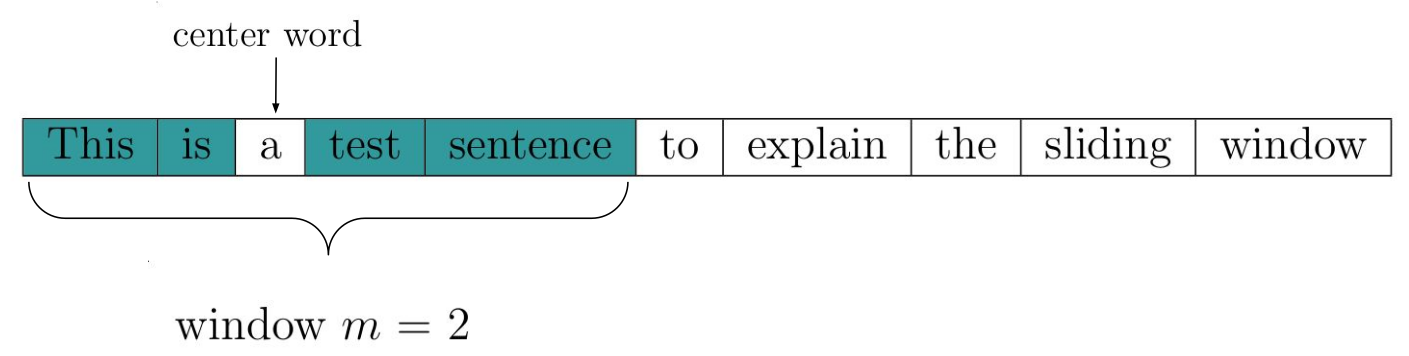
\includegraphics[scale=0.18]{images/window_ex}
\caption{Example of a center word and it's context words}
\label{fig:window_ex}
\end{figure}
With these definitions the fake task can be defined: given a pair consisting of a center and a context words, which will be our training samples, the goal of the network is to predict the probability of each word to appear in the context of the center word. To achieve this goal, Mikolov et al. introduced the following model. The network consists of three layers. See Figure \ref{fig:ntw_architecture} for an illustration. First the network has an input layer, a vector of size $V$ ( $V$ being the size of the vocabulary), represent words as an one hot encoding. Secondly, the projection layer weight Matrix $M_{in}$ stores $V$ $D$-dimensional vectors for the corresponding word in the vocabulary  in it's rows. The projection layer serves as a look up table for our WE (if a one hot vector is multiplied with $M_{in}$ the corresponding WE will result). Finally, the output layer wight matrix $M_{out}$ also stores $V$ $D$-dimensional vector representation of words.The idea behind these 2 Matrices is that the projection layer will represent our words as center word and the output layer as context words. 

\begin{figure}[ht]
\centering
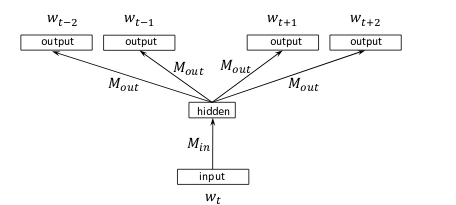
\includegraphics[scale=0.625]{images/ntw_architecture}
\caption{Structure of the network of the Skip Gram Model}
\label{fig:ntw_architecture}
\end{figure}
Since the task of the network being to predict the probability of each word appearing in the context of a given center word, the following probability should be maximized:\\
\begin{equation} \label{eq:basicSkip}
\prod_{i=1}^V \prod_{-m<j<m} p(w_{i+j}|w_i)
\end{equation}
Where $V$ is the number of words in the corpus data, $w_i$ the $i^{th}$ word in the corpus data and $m$ is the context window. This means that the $m$ nearest words to $w$ are considered as context words.
Equation \ref{eq:basicSkip} can be transformed into sums by using log probabilities:
\begin{equation}
\sum _{t=1}^V \sum_{-m<j<m} log( p(w_{i+j}|w_i) )
\end{equation}
where the parameters are the same as in Equation \ref{eq:basicSkip}.

The basic Skip-Gram Model uses a classical Softmax to calculate the conditional probability $p(w_{i+j}|w_i)$:
\begin{equation} \label{eq:softmax}
p(w_{i+j}|w_i)= \frac{exp( \tilde{v}_{w_{i+j}}^Tv_{w_i})}{\sum_{w=1}^V exp(\tilde{v}_w^Tv_{ w_i)}}
\end{equation}

Here $ v_{w_i}$ and $\tilde{v}_{w_i}$ are the vector representations, stored respectively in the projection Layer ($M_{in}$) and in the output layer ($M_{out}$). There is a problem with the classical softmax. For the computation of $\sum_{w=1}^V exp(\tilde{v_w}^T w_t)$, the denominator in Equation \ref{eq:softmax}, one has to go over the whole corpus data. As very big data sets are needed to train the model, this is approach is unsuitable. Mikolov et al. \citep{mikolov2} proposed different solutions. The first solution is to use a Hierarchical softmax introduced by Morin and Bengio \citep{hsoftmax}. In this model, the probability distribution of the output nodes is saved in a binary tree which gives one a logarithmic computation time for each of these probabilities and makes it suitable to compute the softmax. Another possibility is the use of negative sampling which is discussed in the next subsection.

\subsection{Negative Sampling}
A second alternative solution to the use of a classical softmax is negative sampling. Negative Sampling is a simplification of Noise Contrastive Estimation (NCE) which was introduced by Gutmann and Hyv{\"a}rinen \citep{nce-original}, and first applied to NLP by Mnih and Teh \citep{mnih}. This subsection will shortly describe NCE and then how Mikolov et al. \citep{mikolov2} simplified it to create the technique called negative sampling. \\ The idea behind NCE is to distinguish data from noise. It does so by reducing the problem to a logistic regression task and does it by maximizing the log probability. The SGM is only interested in good word representation, hence the probability of the word is not meaningful as long as the quality of the word representations remains high. Mikolov et al. \citep{mikolov2} simplified NCE and called it Negative Sampling, which will be explained next.\\
The main goal of negative sampling is to only update the output nodes of certain words, 5-20 in practice. This will obviously save an enormous amount of computation time. The idea is that given a pair $(c,w) \in D$, wh$w$ ere $c$ is a word in the context window of we select $K$ random words $k_i$ from the corpus data $D$. We assume those words do not appear in the context of $w$. By doing so we will only have to update $k+1$ nodes. Mikolov et al. \citep{mikolov2} introduced the following objective function $J$, that should be maximized:

\begin{equation}
J(c,w)= log(\sigma(v_c \tilde{v_w } ) + \sum_{k\in K} \sigma(log(-v_c \tilde{v_k} ))
\end{equation}\label{eq:obj_neg_samples}

Where $v_c$ and $\tilde{v_w }$, can be interpreted as before in Equation \ref{eq:softmax} and $\sigma(x) = \frac{1}{1+e^{-x}}$. To  understand why this loss function is working so well, one needs to assume that two vectors are similar if their dot product is high. Therefore, we maximize the dot product of similar words $(w,c)$ ($c$ appears in the context of $w$) and minimize it for dissimilar words $(w,k_i)$ (those were selected randomly, we therefore assume that their are not similar).
We see that to compute our objective function we will only have to compute the sum over the number of negative samples $K$, which is very small in practice (2-20). To put things in perspective lets imagine our data set consists of 100000 words, we set $K=2$. Assume each output neuron has a weight vector of dimension $d = 300$. In consequence, when updating our weights we would only update $0.2*10^{-2}$ of the 300 million weights in the output layer.

One question remains: how are the negative samples selected? Mikolov et al. \citep{mikolov2} used the following unigram distribution, to define the probability $P(w)$ of a word $w$ being drawn as a negative sample:

\begin{equation} \label{eq:unigram}
P(w)=\frac{f(w)^{\frac{3}{4}}}{\sum_{t=0}^{T} f(w_t)^{\frac{3}{4}}}
\end{equation}
where $f(w)$ is the frequency of $w_t$. The value of $\frac{3}{4}$ is set empirically. Raising the unigram distribution to the power of $\frac{3}{4}$ makes it less likely for a word to be drawn if it often appears in the dataset in comparison to the basic unigram distribution. See figure \ref{fig:frequency_ex} for an example.\\
\begin{figure}[ht]
\centering
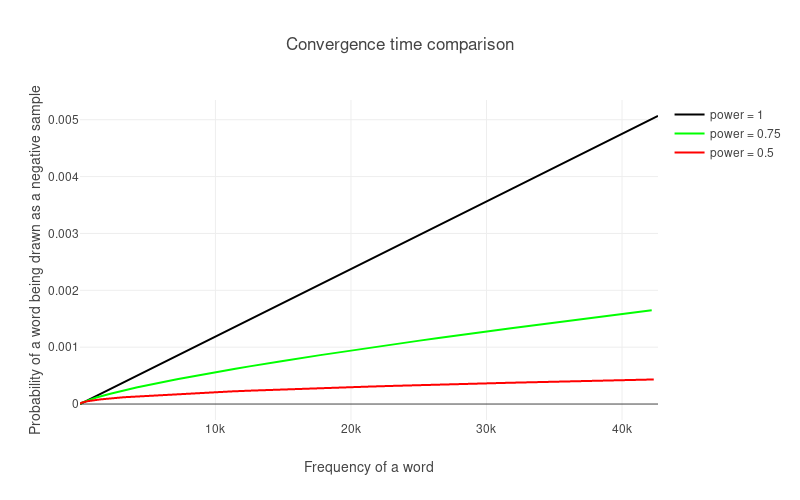
\includegraphics[scale=0.30]{images/frequency_ex}
\caption{Probabililty of a word, of the text8 dataset (sampled), to be chosen at random according to its frequency and the power to which the unigram distribution is raised}
\label{fig:frequency_ex}
\end{figure}
With all of the above knowledge it's understandable that the SGNS will  will outperform the classical softmax in computation time. Now the question arises if the accuracy is maintained but according to Mikolov et al. \citep{mikolov2} the negative sampling method "is an extremely simple training method that learns accurate representations". As a matter of fact, Mikolov et al. \citep{mikolov2} reported a 6\% accuracy improvement in comparison to a Hierarchical Softmax model. Therefore, it is a good solution to the problem raised by the classical softmax.
We now have enough background knowledge about the SGM to look at how it can be optimized. The next section introduces earlier approaches to optimize the SGM.